\documentclass[twocolumn,a4paper,11pt]{article}
\usepackage[utf8]{inputenc}
\usepackage[T1]{fontenc}
\usepackage{amsmath}
\usepackage{amssymb}
\usepackage{graphicx}

\usepackage[margin=2cm]{geometry}

\author{Josh Pattman}
\title{Evolutionary Learning with Extended Mutation Techniques}
\begin{document}
	\maketitle
    \section{Introduction}
    Two of the most important features when describing an organism are its genotype and its phenotype. A genotype encompasses the entire genetic code of an organism, while the phenotype is the physical manifestation of that code as specific traits such as size or color. The relationship between a genotype and a phenotype is a complex one, as a single locus in the genotype does not hold a one-to-one relationship with a single trait in the phenotype. Instead, the phenotype is the result of the entire genotype interacting with the gene regulation network (GRN) of the organism.

    A GRN is a mechanism by which the various genes in the genotype interact by stimulating or repressing each other, eventually resulting in a stable state describing the phenotype. This is an extremely complex process, so for this research, it is simplified to a directed graph. Each node in the GRN graph represents a locus in both the genotype and phenotype, and connections between nodes represent the interactions between genes. The topology of the GRN is not fixed throughout generations, but instead evolves alongside the genotypes of the organisms, with each organism having its own unique GRN. However, the rate of evolution of the GRN is significantly slower than that of the genotype, meaning that the GRN may retain information from previous fitness landscapes, even if that information is not immidiately useful to a given organism at the present time.

    Evolved GRNs have a number of interesting properties. For example, a GRN may recognise genes which frequently covary, and increase the likelihood of those genes being expressed together. A GRN also may take advantage of its ability to retain information to increase the likelihood of a group of traits from a previous landscape being expressed in the future. This is particularly useful in nature, as a previously proven trait of a creature may be more helpful in a future environment than a new randomly evolved one. This ability of a GRN to remember previous fitness landscapes will be reffered to as genetic memory throughout this research.

    This paper aims to investigate the effects of genetic memory in a variety of scenarios, building upon previous work by Richard A. Watson Et al. CITEME, henceforth referered to as the previous work. In the previous work, a specific mathematical model for a genotype and GRN was created, and a hill climbing algorithm was performed to optimise a GRN to commit multiple phenotypes to memory. The trained GRN was then used to produce various combinations of the training phenotypes upon being presented with a random genotypic input.

    The previous work also showed that, using their specific method, the weights of the GRN tended to move towards the weights acheived by Hebbian learning on the training data. This result is significant, as it suggests a hill climbing algorithm may in part be equivalent to more traditional 'intelligent' machine learning algorithms.

    This paper aims to initially reimplement the algorithms of the previous work, and reproduce the results obtained. Following this, an extension to the previous work is proposed, which aims to more accurately model the interactions between genes in a GRN. This extension is then extensively tested and the results are compared to the original work.

    \section{Experiment Setup}
    To represent the genotype of an organism, a vector $G$ is used. This vector has an element per gene in the organism, which in many of the presented cases represents a pixel in an image. Each element can be any in the range $[-1,1]$.

    The GRN is represented by an interaction matrix $B$, which has the same number of rows and columns as there are elements in $G$. The state of the GRN at time $t$ is represented by a vector $P(t)$, which is governed by (\ref{eq:origpa}) and (\ref{eq:origp}). $P(t)$ has no upper and lower bound.
    
    \begin{equation} \label{eq:origpa}
        P(1) = G
    \end{equation}
    \begin{equation} \label{eq:origp}
        P(t+1) = P(t) + \tau_1 \sigma (B P(t)) - \tau_2 P(t)
    \end{equation}
    Where $\tau_1$ and $\tau_2$ are the update rate and decay rate of the network respectively, and $\sigma$ is the $tanh$ function. The final phenotype on which the fitness is evaluated is given by $P(t_{final})$, where $t_{final}$ is set to 10 for all experiments in this paper.

    The fitness function is a modified version of that used in the previous work and is given by (\ref{eqn:fitness}).
    \begin{equation} \label{eqn:fitness}
        |{sum} (P(t_{final}) \odot T)|
    \end{equation}
    In this equation, $T$ is the target phenotype and $\odot$ is the element-wise multiplication operator. Using this function, a value of 0 is minimally fit, but the fitness can extend to positive infinity. The reason for taking the absolute is that a perfect negative of the produced phenotype is indistinguishable from the target phenotype for the GRN. In the previous work, the fitness function would penalise a perfect negative, however this paper chooses to reward it.

    The genetic algorithm (GA) used in this paper is a simple point mutation hill climbing model. At any given time step, there exist two individuals. One of these represents the previous best individual, and the other is a mutated version of the previous best. At each step, the mutated individual is re-initialised to the previous best, then a random point mutation is applied to both its genotype and GRN. If the mutated individual has a higher fitness than the previous best, it becomes the new previous best. This process is repeated for a set number of iterations, and the final best individual is returned. It is imperative that the point mutation size of the GRN is significantly smaller than that of the genotype, otherwise the GRN may overwrite previously learned information. Mutations are either a uniformly or normally distributed random number, which is added to the previous value of the gene.

    \section{Reimplemented Results}
    The first experiment that was reimplemented was experiment 2, shown in Figure 2 in the original work. This experiment aimed to show that the GRN was capable of remembering multiple phenotypes, and was able to reproduce them in future iterations. It also aimed to perform an in depth analysis of the behaviour of the state of the GRN though the timesteps.
    
    For this experiment, SPEAK ABOUT THE EXPERIMENT PARAMETERS.

    Figure \ref{fig:2a} shows how the values of each of the various values of the GRN matrix change thoughout the generations. Each value is represented by a line, with the x-axis representing the generation number and the y-axis representing the value of the matrix. It is clear to see that there are three distinct groups of parameters: increasing, decreasing, and static. The increasing and decreaseing groups are due to the GRN learning either a positive or negative correlation between the genes that cell connects, whereas the static group is due to the GRN learning that the genes are not correlated.
    \begin{figure}[h]
        \centering
        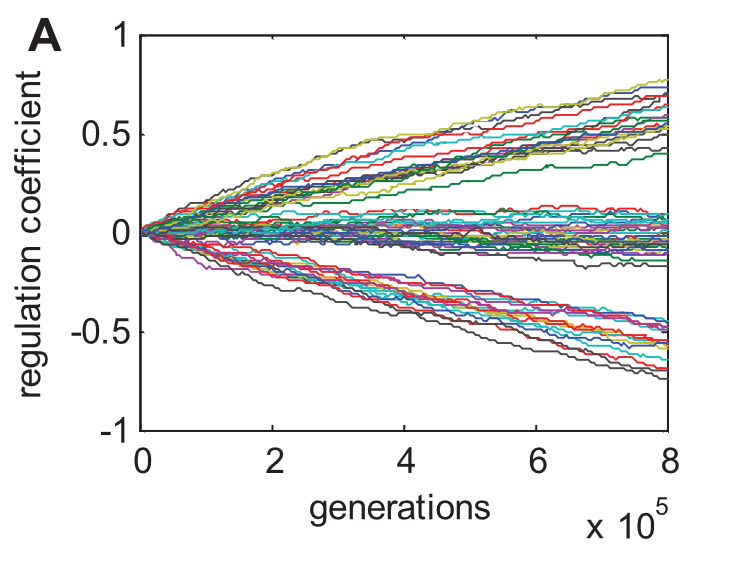
\includegraphics[width=0.48\linewidth]{orig_img/fig2a.png}
        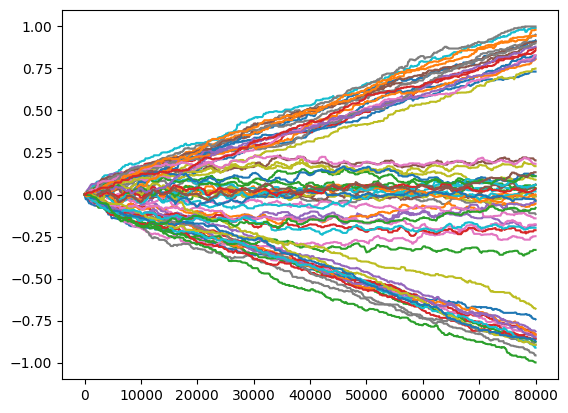
\includegraphics[width=0.48\linewidth]{img/fig2a.png}
        \caption{Values in $B$ over generations. On the left, the original paper. On the right, the reimplemented results.} \label{fig:2a}
    \end{figure}

    Figure \ref{fig:2b} shows a visual representation of the matrix $B$ at the end of training. An identical pattern to that of the original paper emerged, however the weights have a different scale. This is expected, and is due to small changes in the implementation, such as mutation rate. Similarly, Figure \ref{fig:2c} shows the weights obtained using Hebbian learning for $B$. As expected, the weights are very similar to those obtained through hill climbing, suggesting that the hill climbing algorithm may approximate Hebbian learning in this situation.

    \begin{figure}[h]
        \centering
        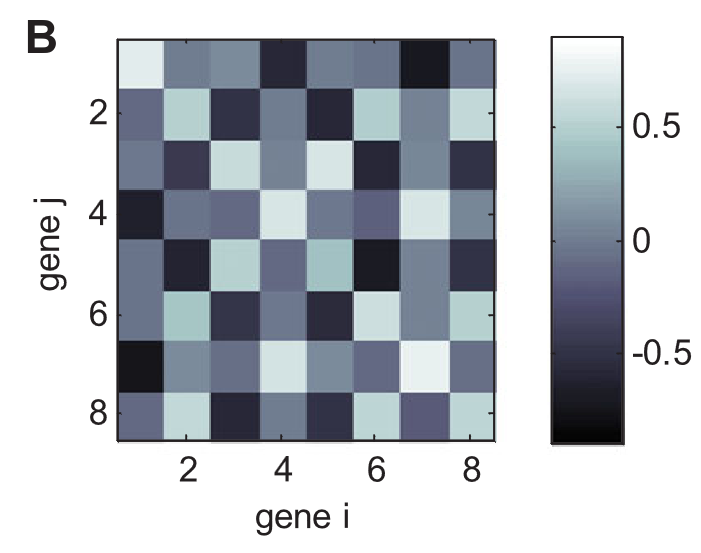
\includegraphics[width=0.48\linewidth]{orig_img/fig2b.png}
        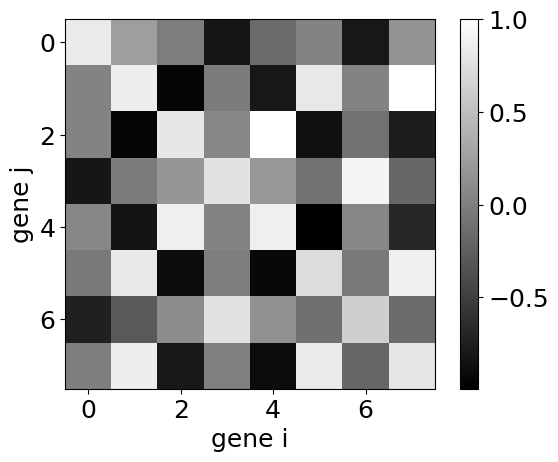
\includegraphics[width=0.48\linewidth]{img/fig2b.png}
        \caption{The final weights in $B$ obtained through a hill climbing process. On the left, the original paper. On the right, the reimplemented results.} \label{fig:2b}
    \end{figure}

    \begin{figure}[h]
        \centering
        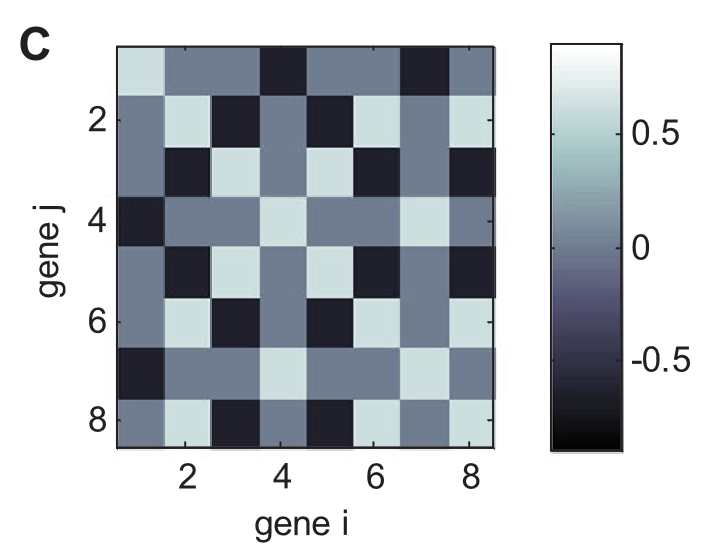
\includegraphics[width=0.48\linewidth]{orig_img/fig2c.png}
        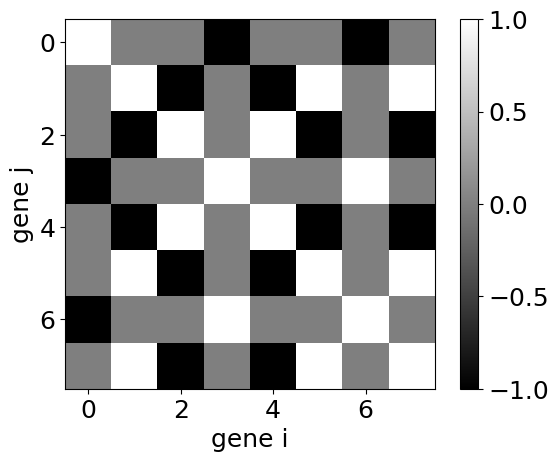
\includegraphics[width=0.48\linewidth]{img/fig2c.png}
        \caption{The weights obtained using Hebbian learning for $B$. On the left, the original paper. On the right, the reimplemented results.} \label{fig:2c}
    \end{figure}

    Figure \ref{fig:2d} demonstrates how the values of $P$ change over the 10 developmental timesteps. Each gene in $P$ is represented by a line, with the x-axis representing the timestep and the y-axis representing the value of the gene. The results presented by this paper clearly follow the same pattern as those from the original work, with the genes all converging to either a stable positive or negative state by the end of the 10 timesteps. There is some correlation between a genes starting value and the state it finally ends up in, but the figure shows that this is not the only factor.

    \begin{figure}[h]
        \centering
        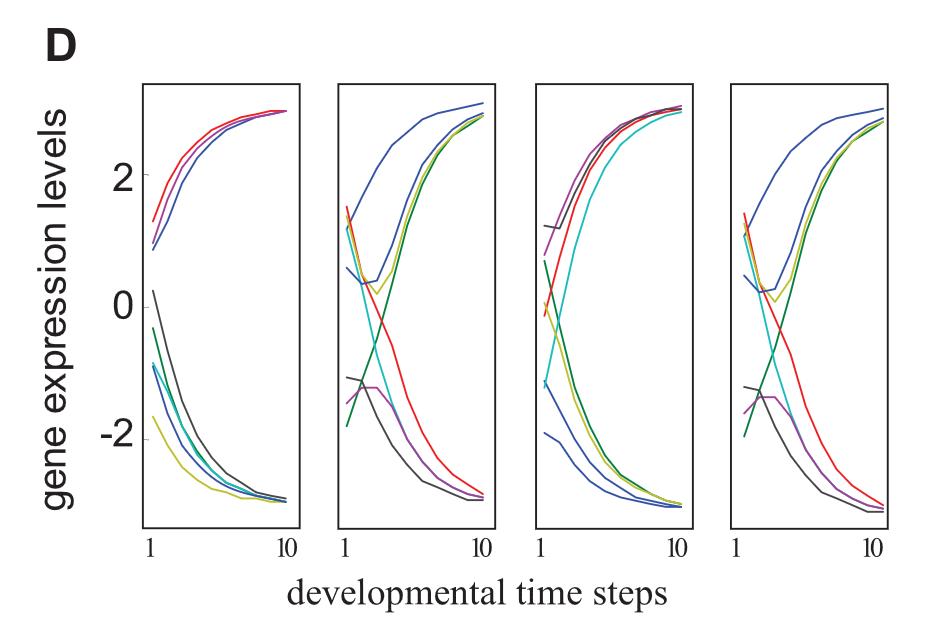
\includegraphics[width=0.9\linewidth]{orig_img/fig2d.png}
        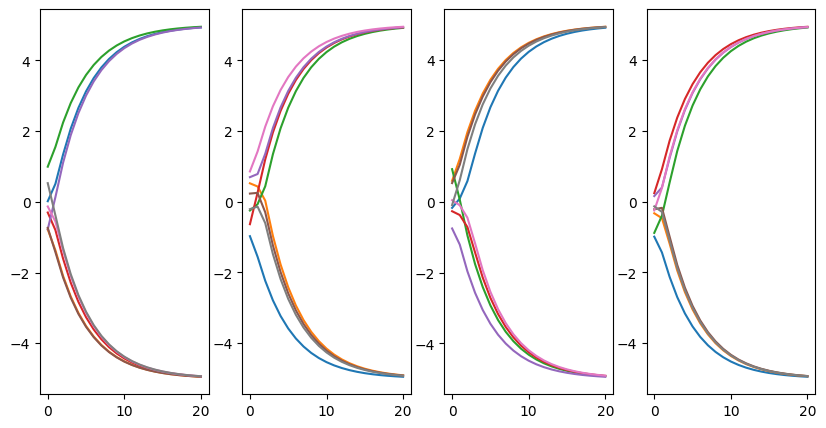
\includegraphics[width=0.9\linewidth]{img/fig2d.png}
        \caption{On the top, the original paper. On the bottom, the reimplemented results.} \label{fig:2d}
    \end{figure}

    Figure \ref{fig:2e} shows a selection of phenotypes produced by the GRN when given a random genotype as input. The results are very similar to those of the original paper, with the GRN producing both targets that are present in the training data. The GRN also produces the inverses of the two targets, which is to be expected.

    \begin{figure}[h]
        \centering
        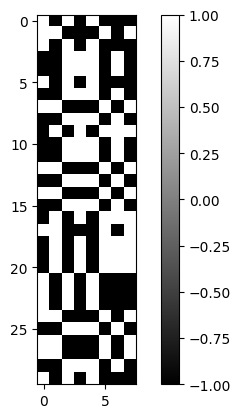
\includegraphics[width=0.45\linewidth]{img/fig2e.png}
        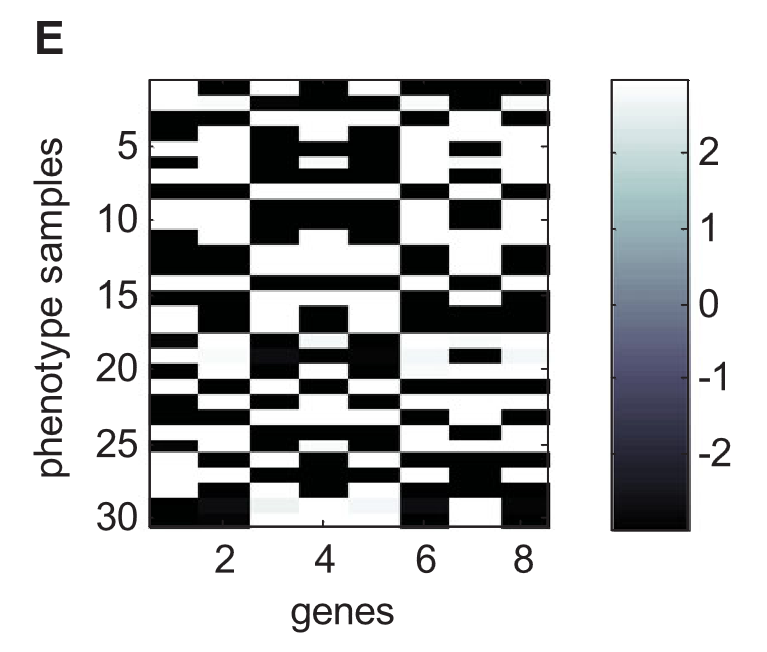
\includegraphics[width=0.45\linewidth]{orig_img/fig2e.png}
        \caption{On the left, the original paper. On the right, the reimplemented results.} \label{fig:2e}
    \end{figure}

    \begin{figure}[h]
        \centering
        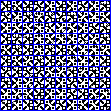
\includegraphics[width=0.45\linewidth]{img/fig4b.png}
        \caption{Bestiary of genotypes reimplemented to the specification of Figure 4 in the original paper.} \label{fig:4b}
    \end{figure}

    \section{Extension}
    The previously descibed model of a GRN provides a significant abstration of the concept of mutations, by modelling a mutation as a small change of the value of the weight between genes. However, this method ignores two other important types of mutation: enabling and disabling connections, and inverting connections.

    When a connection in the GRN is disabled, it maintains its weight but does not contribute to the development of a genotype. However, in the future, this connection may be re-enabled to restore the original weight. This is analogous to rescessive genes in biology, where a gene may still exist but is not expressed in the phenotype of a creature, however that gene may be re-enabled in a descendant of that creature.
    
    Inverting a connection entails reversing the influence of a connection, or in the context of the mathematical model, multiplying the connection by $-1$. This provides the evolutionary process with the ability to quickly reverse the influence of a connection, and therefore the influence which one locus in the genotype has on another. This mutation abstraction has biological parralells with repressor and activator genes, which are the mechanism of GRNs for genes to controll the expression level of each other. Where small incremental mutations such as those implemented by the original work may represent a change in the concentration of a produced activator or repressor, an inversion mutation may signify a switch from a gene producing a repressor to an activator, or vice versa.

    This paper presents a modification to the original model to implement these new mutation types, and hypothesises in the effects of including these. The new mutations are subsequently tested in-depth, and a detailed analysis is given based on the results.

    \subsection{Goals and Hypothesis}
    The aim of the following experiments is to demonstrate the importance of these new types of mutation, and to present evidence for the following hypothesises:


    TODO: I hate the wording of these hypothesis
    \begin{enumerate}
        \item The ability for a GRN to enable and disable genes will be extremely useful for increasing the level of genralisation possible. It has been shown that one of the largest contributors to preventing a GRN from learning genral patterns is the presence of stray connections CITEME. These are introduced in the training set of data, but do not contribute to fitness with thos data samples. The solution to this problem is to encourage the GRN to use as few weigths as possible to achive a maximal fitness, which has been implemented using an L2 normalisation term in the past CITEME. However, with the process of disabling genes being so simple for the GRN with this type of mutation, the amount of stray connections may drasically reduce, especially if also paired with a normalisation term.
        \item The GRN may find local optima easier to escape due to the ability for flip connections to occur, enabling much larger changes in its behaviour. One of the common issue with a trained GRN is that single pixels may be confidently expressed as the incorrect color. It may be simpler for the GRN to flip these when a weight inversion is possible.
    \end{enumerate}

    \subsection{Model}
    The aims of producing a model for the updated GRN were two-fold. Firstly, the extended model should introduce as little extra complexity as possible, which would not only maintain fast simulation times but also ensure the model would not stray too far from its biological inspiration. Secondly, the model should maintain maximum similarities to the original, maintaining easy comparisons between the structure and performance of the two.

    The presented model, formalised in Equations \ref{eq:extenda} and \ref{eq:extendb}, furfills both of these requirements. In Equation \ref{eq:extendb}, the $*$ symbol represents element-wise matrix multiplication, the matrix $B_s$ is the sign matrix, and $B_m$ denotes the magnitude matrix. The sign matrix contains values in the set $\{-1,0,1\}$, however the magnitude matrix may contain any values. All other symbols hold the same meaning as those in Equation \ref{eq:origp}.

    \begin{equation} \label{eq:extenda}
        P(1) = G
    \end{equation}
    \begin{equation} \label{eq:extendb}
        P(t+1) = P(t) + \tau_1 \sigma ((B_s * B_m) P(t)) - \tau_2 P(t)
    \end{equation}

    Mutations on this model are applied with a differnt process to that of the original. Firtly, the matrix to mutate is randomly chosen with a probability which heavily favours the matrix $B_m$. In the following experiments, the chance of mutating $B_s$ was $0.1\%$. If $B_m$ was chose, mutations are applied as descibed in the original model. However, if $B_s$ is chose to be mutated, a random cell of the matrix is changed to a value chosen unformly from the set $\{-1,0,1\}$, irrespective of what the cell's value was before.

    \section{Extension Results}
    \begin{itemize}
        \item 1.5 page
    \end{itemize}

    Compare bestiary of dense to bitdense

    Compare different number of proteins

    Compare number of parameters

    Compare training speed


    \section{Conclusion}
    This study has not only shown the reproducibility of the results obtained by R. Watson et al \cite{rich}, but has also contributed some valuable insights into improvements which can be made upon the model of a GRN.

    \begin{itemize}
        \item This paper has presented results which agree with the original conclusion that the hill climber tends towards the hebbian weights.
        \item However, upon implementation of the extension, it was shown that similar results could be obtained even with significanty different weights to the hebbian ones.
        \item This may suggest that the hill climbing algorithm is not as similar to hebbian learning as previously thought, or that the extension model is not as effective as the original model.
        \item The extension model was also shown to be faster training and more robust than the fully dense network.
        \item A major critique of this method is that the weights of -1, 0, and 1 are straying quite far from real-life biology, where each gene may release a concentration of a certain protein.
        \item However, the aim of these experiemnts was never to make a perfect biological model, but instead a rough approximation which could be used to explore the effects of genetic memory in a GRN.
        \item Bitdense is also very sensitive to learnging rate, bit probability, and generations before switch, making it harder to tune and get right
        \item Running some sort of meta hill climber than runs multiple bit dense sims at once, each with own learning rate, and has competition between different sims may be future work, allowing the optimal params to be found.
        \item It is also very possible to come up with better but less biologically training algorithms, which may be interesting to explore in the future (some sort of GAN-inspired architechture / competitive coevolution)
    \end{itemize}


    \section{Appendix}


\end{document}